\chapter{Research}

This chapter gathers all research information together which is necessary to create and validate a functioning NLP model. This
isn't only about choosing the right algorithms for the task but also about finding ways to compare multiple approaches against
each other and validating their results.

\section{Performance Metrics}
\label{chap:formulas}
There exist several performance indicators each data scientist should be aware of. These specific metrics are used to validate
the outcome of models and make different solutions comparable. As in figure \ref{fig:metrics} displayed, there is a basic
concept which these metrics are build on top of.

\begin{figure}[!ht]
\centering
\frame{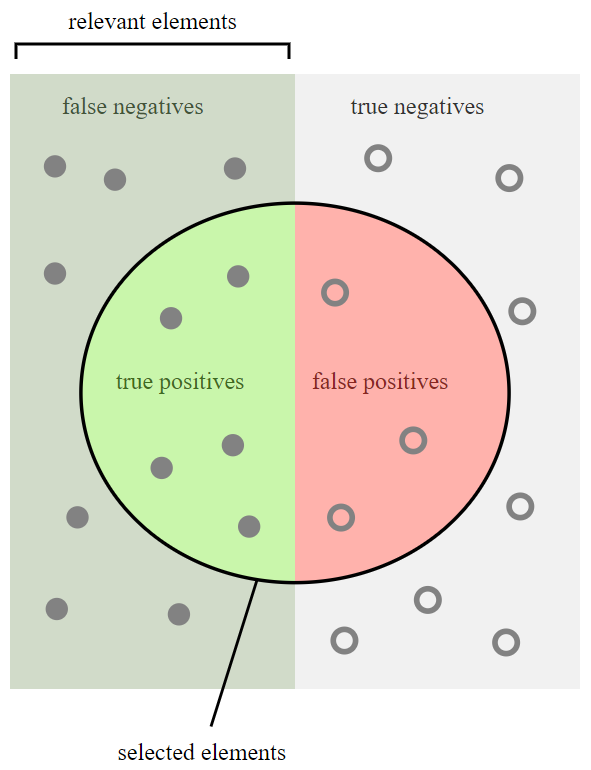
\includegraphics[scale=0.4]{metrics-overview}}
\caption{Overview about possible classification outcomes\cite{wiki01}}
\label{fig:metrics}
\end{figure}

For every classification task there exist exactly four possible outcomes. When the model classifies an element correctly it's
either a \emph{true positive} or a \emph{true negative} value. The keyword \emph{true} relates to the assumption the model did.
Vice versa it's either a \emph{false positive} or a \emph{false negative} value if the model's assumption is wrong.

The combination of \emph{true positive} and \emph{false negative} values is the amount of relevant data we want to have a closer
look on. For example this could be a set of \emph{named entities} or a group of patients which have a certain disease.

\subsection{Why Accuracy is not enough}

Probably the most well-known and certainly the easiest metric to understand is called \emph{accuracy}. It describes the
closeness of a set of predictions to its corresponding \emph{truth values}. Accuracy is the proportion of all correctly classified
elements in relation to the total quantity. It's value lies somewhere between zero and one.

\begin{equation}
    \label{math:accuracy}
    accuracy = \frac{\textit{true positives} + \textit{true negatives}}{\textit{total population}}
\end{equation}

There is one large downside with accuracy which makes it useless for many classification problems. If there's one category
representing the majority of elements, accuracy will always be at a very high level. This is called an \emph{imbalanced
classification problem} \cite{koehrsen}. Imagine a model for detecting very rare diseases which simply labels each tested patient
as \emph{negative}. If the chance of getting this disease is about \(\frac{1}{10000}\), the accuracy of such model would be at
stunning $99.99\%$. That's why every data scientist should consider using more advanced metrics like described in the next section.

\subsection{Precision and Recall}

\emph{Precision} measures the accuracy of the positive predictions. In other words, it's the proportion of correctly classified
elements in relation to all elements the model marked as \emph{positive}. A model which randomly classifies a single element as
\emph{positive} and is right about that, will have a \emph{precision} of $1.0$. The results of a model with a high \emph{precision}
are very useful because most values have been correctly classified and therefore can be used for further processing.

\begin{equation}
    \label{math:precision}
    precision = \frac{\textit{true positives}}{\textit{true positives} + \textit{false positives}}
\end{equation}

\emph{Recall}, or sometimes called \emph{sensitivity}, is the number of correct classifications compared to the number of elements
which should have been found in total. A \emph{recall} of $100\%$ can simply be achieved by classifying every element as \emph{positive}.
Therefore it should be combined with \emph{precision} to get an expressive statement about the model performance.

\begin{equation}
    \label{math:recall}
    recall = \frac{\textit{true positives}}{\textit{true positives} + \textit{false negatives}}
\end{equation}

There is a trade-off between the two metrics \emph{precision} and \emph{recall}. An optimization which increases the \emph{recall}
will likely decrease the \emph{precision} and vice versa. If neither \emph{recall} nor \emph{precision} is more important, there
exists the \emph{F1 score} (\ref{math:f1}) which is the harmonic mean of both. The mean itself isn't very meaningful because if the
model performs very good at one metric and poorly at the other, it will be still around $0.5$. The harmonic mean punishes low values
and doesn't compensate them with high values for the opposite metric. In many cases, \emph{F1 score} is a good metric to describe the
overall performance of a model \cite{Grus15}.

\begin{equation}
    \label{math:f1}
    \textit{f1 score} = 2 * \frac{precision * recall}{precision + recall}
\end{equation}

\section{Named-entity Recognition}

\acrfull{ner} is the first and probably most important discipline of \emph{information extraction}. Its goal is to detect
\emph{named entities} which is roughly everything that has a proper name. Sometimes this group is extended with terms like prices,
dates and times \cite{Jurafsky2000}. It's common to create own domain specific entities, e.g. an entity type \emph{insurance} which
might be useful for the Swiss Mobiliar. Table \ref{tbl:named-entities} shows typical named entity types which are supported by a
large variety of \acrshort{ner} libraries. \emph{Locations} and \emph{geo-political entities} are sometimes combined\footnote{The NLP
library spaCy combines these two for models trained by the Wikipedia corpus}.

\begin{table}[h!]
    \centering
    \begin{tabular}{|l|l|l|}
        \hline
        \textbf{Type} & \textbf{Tag} & \textbf{Description} \\ [0.5ex]
        \hline
        People & PER & People, Characters \\
        Organisation & ORG & Companies, NGOs, Sports \\
        Locations & LOC & Regions, Mountains, Seas \\
        Geo-Political Entity & GPE & Countries, Cities, Provinces \\ [1ex]
        \hline
    \end{tabular}
    \caption{List of generic named entity types}
    \label{tbl:named-entities}
\end{table}

Entities are used to recognise relations between people or for question answering like Google does\footnote{Simply google "who's
the mother of Zeus" where "Zeus" is a named entity}. Another possible use case is the automated grouping of news articles by
referenced people, organisations or locations \cite{gupta}.

\subsection{Difficulties}

In \acrlong{ner} it can be very difficult to decide what's a named entity and what's not. The term \emph{general agency Berne} can
refer to an organisation whereas the token \emph{Berne} could reference the capital of Switzerland. For the best possible results
it's important to define the boundaries of what's a named entity and what's not and to be strict while labelling.

Another difficulty is if you have to deal with word ambiguity. Imagine the entity \emph{Orange} which can either be a fruit, a colour,
a telecommunication provider or a city in France. Many fashion labels are named after designers like \emph{Calvin Klein} or \emph{Ralph
Lauren} but when people mention them, they mostly mean the brand rather than the actual person \cite{Vogel19}. The \acrshort{nlp} model
needs to concern the context in which the ambiguous term occurred to give a solid prediction.

\subsection{Labelling Standards}

Named entities need to be described in a standardised way so that \acrshort{ml} models can interpret them. There exist a few labelling
standards which are often used in \acrshort{ner}. If you have to chose a specific labelling standard, keep in mind that sophisticated
labelling techniques give you more information than e.g. binary labelling. You can always downgrade to a lower standard but getting
distinctive labels out of binary tags isn't possible. On the other hand, it's often easier to label data with low-level tags rather
than e.g. \acrshort{iob} tags.

\subsubsection{Binary}

Binary tagging is the simplest form of labelling. Every token which isn't a named entity is going to be labelled as $0$. The remaining
tokens which are all entities are tagged with $1$. If multiple label types need to be distinguishable, binary tagging isn't the preferred
method. As you can see in table \ref{tbl:binary-labelling}, the two entities \emph{people} and \emph{food} cannot be distinguished.

\begin{table}[h!]
    \centering
    \begin{tabular}{|c|c|c|c|c|c|c|c|}
        \hline
        Bond & drinks & his & vodka & martini & shaken, & not & stirred. \\
        \hline
        1 & 0 & 0 & 1 & 1 & 0 & 0 & 0 \\
        \hline
    \end{tabular}
    \caption{Example of a binary tagged sentence}
    \label{tbl:binary-labelling}
\end{table}

\subsubsection{IOB (Inside-outside-beginning)}

Unlike binary tags, \acrshort{iob} labels allow you to differentiate between multiple label types. \emph{Bond} and \emph{vodka martini}
are clearly not in the same entity group (\ref{tbl:iob-labelling}). Additional to the variable types, \acrshort{iob} tagging indicates
multi-token entities as such. In the \emph{IOB2} format, the first token of a sequence is always labelled with the prefix \emph{B-} for
beginning, the rest with an \emph{I-} for inside \cite{bio95}.

\begin{table}[h!]
    \centering
    \begin{tabular}{|c|c|c|c|c|c|c|c|}
        \hline
        Bond & drinks & his & vodka & martini & shaken, & not & stirred. \\
        \hline
        B-PER & O & O & B-FOOD & I-FOOD & O & O & O \\
        \hline
    \end{tabular}
    \caption{Example of an IOB tagged sentence}
    \label{tbl:iob-labelling}
\end{table}

As shown in table \ref{tbl:iob-labelling2}, the first two tokens are from the same type but still distinguishable. With binary tags you
would most likely interpret both tokens as one large named entity consisting of two separate words.

\begin{table}[ht!]
    \centering
    \begin{tabular}{|c|c|c|c|c|c|}
        \hline
        Huey, & Dewey, & and & Louie & are & triplets. \\
        \hline
        B-PER & B-PER & O & B-PER & O & O \\
        \hline
    \end{tabular}
    \caption{Example of distinctive beginning tags}
    \label{tbl:iob-labelling2}
\end{table}

The \acrshort{iob} format was later extended by an indicator for single and ending tokens. It's called \emph{BIOES} and can be useful if
tokens are processed separately from each other so that the model cannot be able to recognise multi-token values by itself \cite{hofer18}.